\documentclass{article}
\usepackage[T1]{fontenc}
\usepackage{lmodern}
\usepackage{graphicx}
\usepackage{amsmath,amssymb}
\usepackage[a4paper,margin=2cm]{geometry}
\usepackage[absolute,overlay]{textpos}
\setlength{\TPHorizModule}{1mm}
\setlength{\TPVertModule}{1mm}
\usepackage[indonesian]{babel}
\usepackage{hyperref}
\setlength{\emergencystretch}{2em}
% unit: Halaman 71

\begin{document}

% === Halaman 71 (llm) ===

Kunci dapat dipilih dari sebuah kalimat yang mudah diingat, misalnya:

\begin{center}
JALAN GANESHA SEPULUH
\end{center}

Buang huruf yang berulang dan huruf $J$ jika ada:

\begin{center}
ALNGESHPU
\end{center}

Lalu tambahkan huruf-huruf yang belum ada (kecuali $J$):

\vspace{69.50mm}

\begin{center}
ALNGESHPUBCDFIKMOQRTVWXYZ
\end{center}

Masukkan ke dalam bujursangkar:

\vspace{10mm}

% deskripsi: Tabel bujursangkar yang berisi huruf-huruf hasil proses penyusunan kunci kriptografi.
% bbox normalisasi: [0.3170, 0.6530, 0.5120, 0.8870]
\begin{textblock*}{40.95mm}(66.57mm,193.94mm)
\noindent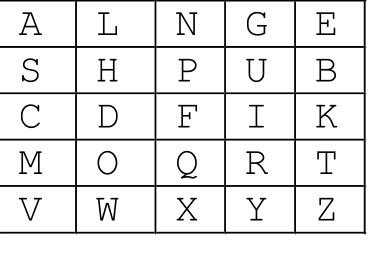
\includegraphics[width=40.95mm,height=69.50mm]{../../images/llm/page_071_img_01.png}%
\end{textblock*}

\end{document}
